%%%%%%%%%%%%%%%%%%%%%%%%%%%%%%%%%%%%%%%%%
% Short Sectioned Assignment
% LaTeX Template
% Version 1.0 (5/5/12)
%
% This template has been downloaded from:
% http://www.LaTeXTemplates.com
%
% Original author:
% Frits Wenneker (http://www.howtotex.com)
%
% License:
% CC BY-NC-SA 3.0 (http://creativecommons.org/licenses/by-nc-sa/3.0/)
%
%%%%%%%%%%%%%%%%%%%%%%%%%%%%%%%%%%%%%%%%%

%----------------------------------------------------------------------------------------
%	PACKAGES AND OTHER DOCUMENT CONFIGURATIONS
%----------------------------------------------------------------------------------------

\documentclass[paper=a4, fontsize=11pt]{scrartcl} % A4 paper and 11pt font size

\usepackage[T1]{fontenc} % Use 8-bit encoding that has 256 glyphs
\usepackage{fourier} % Use the Adobe Utopia font for the document - comment this line to return to the LaTeX default
\usepackage[english]{babel} % English language/hyphenation
\usepackage{amsmath,amsfonts,amsthm} % Math packages
\usepackage[margin=1.25in]{geometry}

\usepackage{listings}
\usepackage{graphicx}

\usepackage{lipsum} % Used for inserting dummy 'Lorem ipsum' text into the template

\usepackage{sectsty} % Allows customizing section commands
\allsectionsfont{\centering \normalfont\scshape} % Make all sections centered, the default font and small caps

\usepackage{fancyhdr} % Custom headers and footers
\pagestyle{fancyplain} % Makes all pages in the document conform to the custom headers and footers
\fancyhead{} % No page header - if you want one, create it in the same way as the footers below
\fancyfoot[L]{} % Empty left footer
\fancyfoot[C]{} % Empty center footer
\fancyfoot[R]{\thepage} % Page numbering for right footer
\renewcommand{\headrulewidth}{0pt} % Remove header underlines
\renewcommand{\footrulewidth}{0pt} % Remove footer underlines
\setlength{\headheight}{13.6pt} % Customize the height of the header

\numberwithin{equation}{section} % Number equations within sections (i.e. 1.1, 1.2, 2.1, 2.2 instead of 1, 2, 3, 4)
\numberwithin{figure}{section} % Number figures within sections (i.e. 1.1, 1.2, 2.1, 2.2 instead of 1, 2, 3, 4)
\numberwithin{table}{section} % Number tables within sections (i.e. 1.1, 1.2, 2.1, 2.2 instead of 1, 2, 3, 4)

% \setlength\parindent{0pt} % Removes all indentation from paragraphs - comment this line for an assignment with lots of text

%----------------------------------------------------------------------------------------
%	TITLE SECTION
%----------------------------------------------------------------------------------------

\newcommand{\horrule}[1]{\rule{\linewidth}{#1}} % Create horizontal rule command with 1 argument of height

\title{	
\normalfont \normalsize 
\textsc{Experimental Methods in Perception} \\ [25pt] % Your university, school and/or department name(s)
\horrule{0.5pt} \\[0.4cm] % Thin top horizontal rule
\huge Final Project : \\ Visual Search Time in Identifying Cyclists \\ % The assignment title
\horrule{2pt} \\[0.5cm] % Thick bottom horizontal rule
}

\author{Ammon Pekes and Armon Shariati} % Your name

\date{\normalsize\today} % Today's date or a custom date

\begin{document}

\maketitle % Print the title

\section{Introduction}

%% Visual search is a task in which the subject in an experiment is asked to
%% identify a target item amongst a sea of distractor items. Researchers designing
%% visual search experiments, such as ourselves, are usually interested in the time
%% it takes for the subject to find the target. It is not hard to imagine that
%% tasks end up falling into one of two categories: ``pop-out'' and ``serial
%% search''. In the first case, the target is readily apparent, and the response
%% time of the subject is independent of the number of distractors. In the latter
%% case, the target is better hidden, and the subject must examine each item in a
%% sequence. As a result, reaction time increases with the number of distractors,
%% and the increase per distractor is double per ``no'' responses than for ``yes''
%% responses. 
%% 
%% 
%% In our experiment, we were primarily interested in the amount of time it takes
%% for a subject to identifying a cyclist through varying amounts of visual
%% ``clutter''. Furthermore, we were interested in seeing if and how different
%% colored tail lights on a cyclist would affect the time it takes for a subject
%% to identify them. 


An estimated 48,000 cyclists were injured in motor vehicle traffic accidents in
2013, over half of which occurred in low light conditions \cite{nhtsa2015}.
Drivers often fail to observe cyclists, making cyclists particularly vulnerable
\cite{wood2013bicyclists}. Visual Search studies provide insight into why this occurs.
Visibility is certainly an issue: bike lights are often quite dim in comparison
to car lights, and the intensity of the signal predictably influences
performance [Engel, 1977]. Attention also dramatically alters perception. Since
bikers represent rare events, drivers are not attentive to their presence.
Additionally, visual search is influenced dramatically by the azimuth
\cite{treisman1980feature}. A bike in a bike lane falls somewhere between
$30^\circ-90^\circ$ lateral of the usual center of vision of a driver.
Visual acuity drops dramatically as eccentricity increases, making cyclists
potentially invisible to drivers \cite{wolfe1998there}. 

Here we seek to determine how color affects biker recognition in a
pseudo-realistic context. Because of the variety of factors involved, we
developed an experimental procedure to test visual search for bikers against a
backdrop of natural scenes filled with common distractors: cars, billboards,
street lamps, and stop lights.

\section{Methods}

Using \texttt{Python} in hand with its \texttt{OpenCV} bindings, we created a
program the generates a sequence of images which resemble what a motorist would
likely see while driving through rural, highway, and urban environments. After buffering
the series of images, the program presented the images to a subject. In exactly
half of the images a subject encountered, a cyclist was present with a
different colored tail light. Furthermore, the subject was tasked with finding
a cyclist if one was present, and then to respond in the affirmative if that
was the case. The program records the subjects response as well as the time it
took them to do so.

\smallskip
The images with cyclists in them are synthetic and are constructed in 
a two part process as follows. An example can be seen in Figure \ref{fig:scene}.

\begin{enumerate}

    \item We took two photographs of cyclists found online and using
        \texttt{Adobe Photoshop and Illustrator} we manually cropped out
        everything except the cyclist itself, and then decreased the $\alpha-$
        value making the cyclist look slightly transparent. This was done to
        ensure better blending in the final result. We chose two photographs
        where one cyclist was wearing very bright clothing and one where a
        cyclist was wearing darker clothing. Since we were primarily concerned
        with the affect of the tail light color, we wanted to make sure the
        data reflects any effects of the clothing color on response time as
        well.  For each of the two cyclists images, we created $8$ copies and
        drew a fully visible (max $\alpha-$ value) ``blob'' of a different
        color in the approximate location of where a tail light for a cyclist
        would likely be situated - one copy is left unmodified as a control.
        Therefore, in total there were $16$ unique cyclist images. 

    \item The program reads in each of the $16$ cyclist images, and places it
        within an image still from dash-cam footage captured at night.  The
        location at which the cyclist is placed is chosen at random, but
        constrained to be within the inner $75\%$ of the background image. The
        stills are hand selected from the footage and are chosen in an attempt
        to capture a myriad of lighting conditions, clutter, and perspective.

\end{enumerate}

\vspace{2mm}
\begin{figure}[h!]
    \label{fig:scene}
    \centering$
    \begin{array}{cc}
        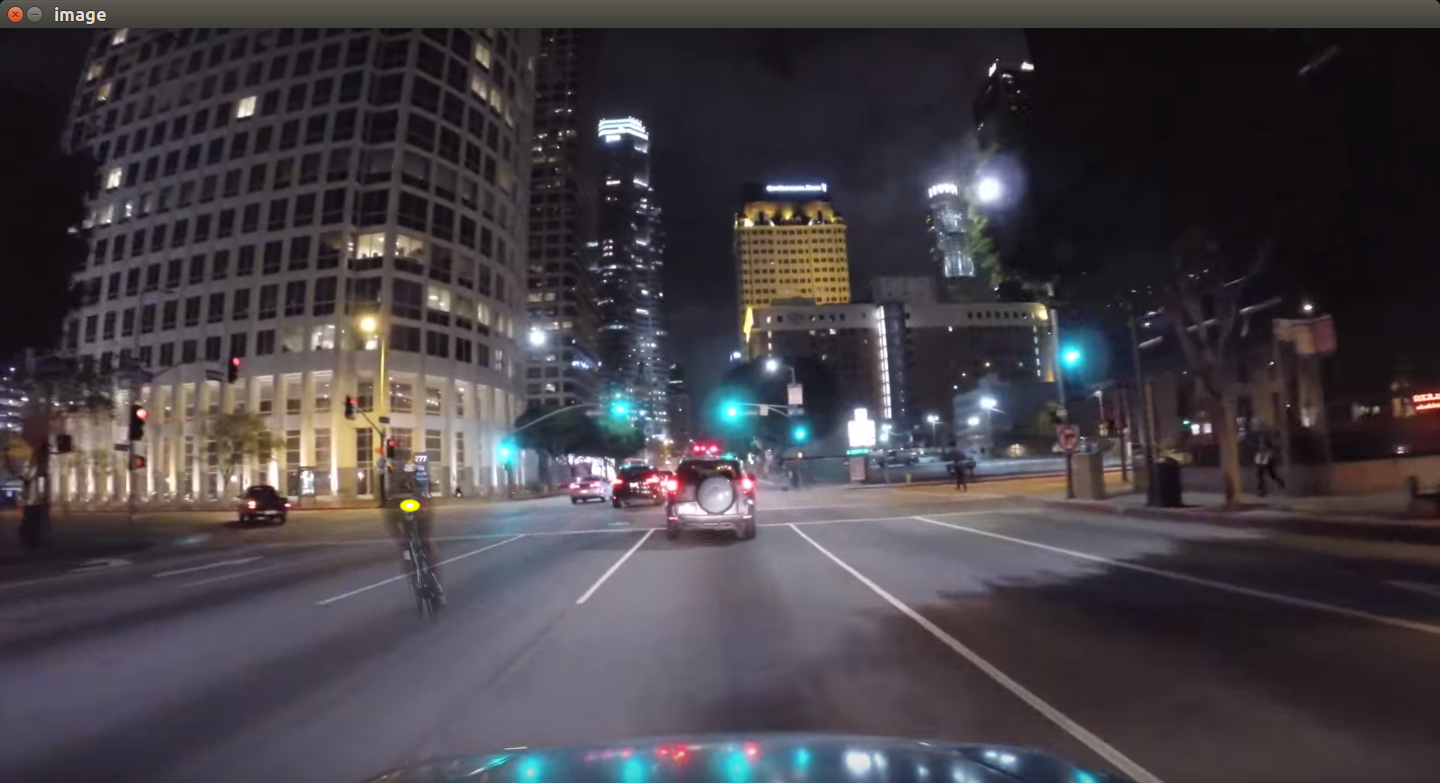
\includegraphics[width=0.8\textwidth]{figures/yellow1.png} \\
        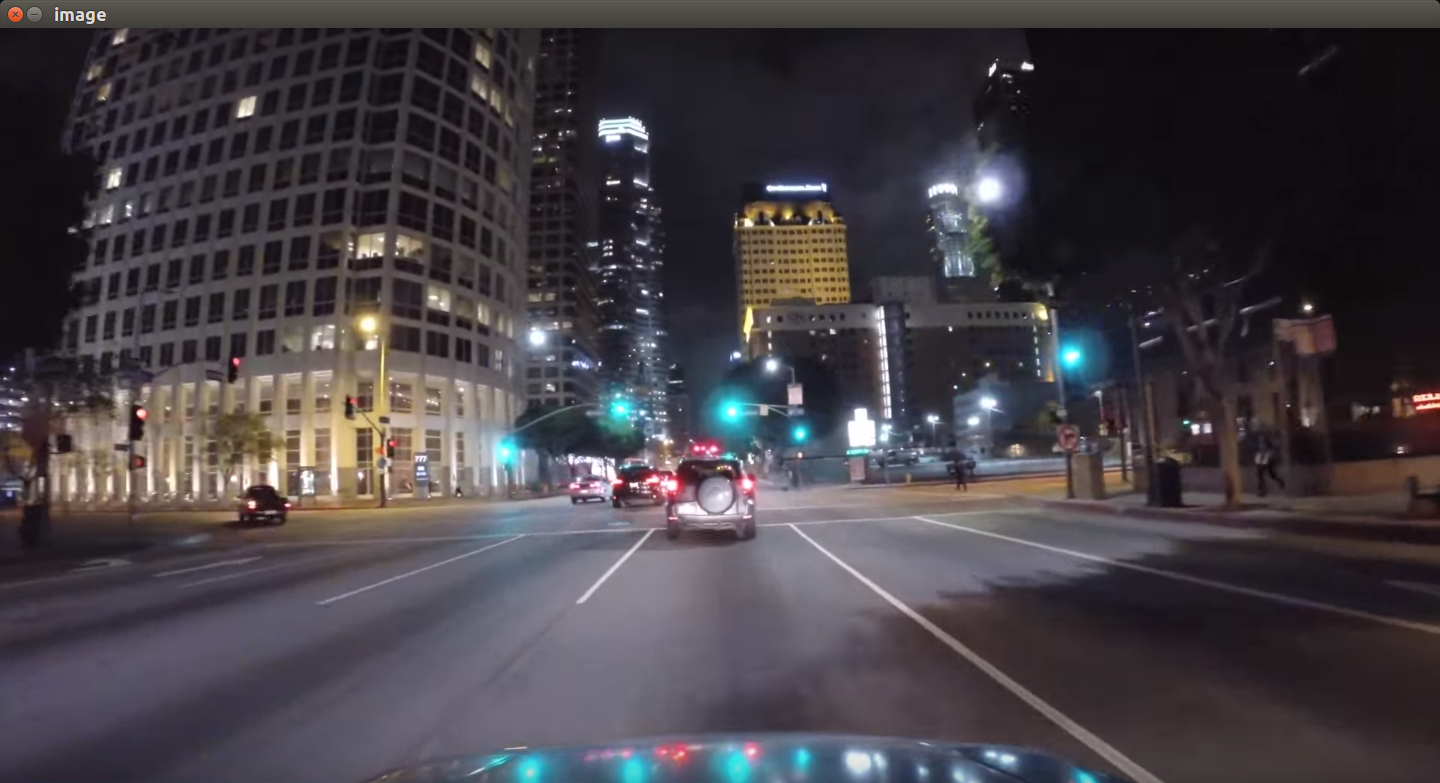
\includegraphics[width=0.8\textwidth]{figures/city1.png}
    \end{array}$
    \caption{ A dash-cam still with and without the embedded cyclist. }
\end{figure}





\end{document}
